
\chapter{Background}
\label{cha:background}
This chapter will discuss the main topics needed to understand this work, from
discrete event systems to discrete control implementation on \PLCs, a more
detailed explanation of each topic can be found on the respective cited work.
\section{Systems}

A System as defined by the Cambridge's dictionary is ``a set of connected
things or devices that operate together''. As seen two basic properties
of systems
are :
\begin{itemize}
\item they are formed by grouping smaller parts
\item the smaller parts when grouped work together to carry out a specific function
\end{itemize}

As its definition is so abstract almost anything can be defined as a system,
physical or not, beings can be defined as systems and even economic mechanisms
can also be considered as systems.

Usually systems are modeled by a Input/Output process. The system is fed with a
set of inputs, it process the inputs resulting on the output set, as we can see in  \autoref{fig:ioProcModel}. 

\figplaceholder{Input/ Output Process model}{ioProcModel}

In some systems, its inputs and outputs can't represent it's behavior, so
the concept of state is created, and it represents the behavior of the system in
a given instant $t$.

The states can be continuous or discrete, and the systems which these states
represent can be considered as Continuous Systems, Discrete Systems or even
Hybrid Systems, which combine both kind of states.

The systems modeled in this work are Discrete Systems, more details about other
kinds of systems as well as examples and their analysis can be found on \cite{oppenheim1996signals}
and \cite{kalouptsidis1997signal}.
\section{Discrete Event Systems}
\label{sec:discreteEventSystems}
Discrete Systems can be driven by time and by events. It means, the states can
be changed continuously by the time or some external event can interfere at a
given instant. 

In this thesis we are interest in the event-driven type. Some basic mathematical
formalisms, nomenclature and representations can be
developed to facilitate the understanding. Some of those will be presented in
the following subsections based on \cite{cassandras2009introduction}:
\subsection{Languages}
\label{sec:automata}
A language can be defined by the Merriam-Webster's dictionary as ``a systematic means of communicating ideas or feelings by the use of conventionalized signs, sounds, gestures, or marks having understood meanings''
And as it is defined by this dictionary entry we pursue to communicate the complete
behavior of the \DES.
Firstly we need to define a group, or
set of marks to characterize the singular behavior of the system.
So, we define a
set $\Sigma$. This set contains all elements which combined can create a language.
Again in analogy with linguistics, each one of these marks, the events can be
compared to
letters
, provided that $\Sigma$ can be called an ``alphabet'', and the combination of
its events ``words''. We can also define a mark to represent an empty word,
$\epsilon$, that is, a word that is not formed by any event.

Likewise, we can define the length of a word as the number of events contained by
this word, we denote the length with two vertical bars, given a word $s$ its
length is equal to $|s|$ and by definition $|\epsilon| = 0 $.

As we know, there is a great number of human western languages, as portuguese, english,
french, spanish etc, that roughly are formed by the same alphabet, but overall
they are formed by different combination of words.  
Similar things can happen with languages that define the \DESs, so we can define
as in \cite{cassandras2009introduction}.

\begin{definition}[Language]
\label{def:language}~\\  
A Language defined over an event set $\Sigma$ is a finite-length set formed from
events in $\Sigma$
\end{definition}

Take for example an alphabet $\Sigma = \{\}$WAs
\subsection{Automata}
\label{sec:automata}
\begin{definition}[Deterministic Automaton]
\label{def:DeterministicAutomaton}~\\  
A Deterministic Automaton, denoted by G, is a five-tuple
\[ G = (X,\Sigma,f, x_0,X_m)\]
where:

\indent X is the set of \textbf{states} \\
\indent $\Sigma$ is the finite set of \textbf{events} associated with G\\
\indent f: X $\times \Sigma \rightarrow X$ is the \textbf{transition function}  \\ 
\indent $x_0$ is the \textbf{initial state} \\
\indent $X_m \subseteq X $ is the set of \textbf{marked states}

\end{definition}
\todo{

As in \cite{cassandras2009introduction} the initial states on this thesis are
going to be identified by an arrow pointing towards them, and marked states by
double circles.

\begin{figure}[H]
  \centering
  \includegraphics[width=0.5\textwidth]{automata/example/example.tikz}
  % \includetikzfigure[width=0.5\textwidth]{automata/example/example}
  \caption{Diagram representing the Automata from example number }
\end{figure}


\subsubsection{DAOCT}

\begin{definition}[Deterministic Automaton With Outputs and Conditional
  Transitions (DAOCT)]
\label{def:daoct}~\\  
A Deterministic Automaton, denoted by DAOCT, is a nine-tuple
\[ DAOCT = (X,\Sigma,f,\lambda,R,\theta, x_0,X_f)\]
where:

\indent X is the set of \textbf{states} \\
\indent $\Sigma$ is the finite set of \textbf{events}\\
\indent $\Omega \subset \mathbb{N}_1^{m_i+m_o} $ is the set of \textbf{I/O vectors}\\
\indent f: X $\times \Sigma^\star \rightarrow X$ is the \textbf{deterministic transition function}  \\ 
\indent $\lambda : X \rightarrow \Omega$ is the \textbf{state output function} \\
\indent $R = {1,2,\dots,r}$ is the set of \textbf{path indices} \\
\indent $\theta : X \times \Sigma \rightarrow 2^R$ is the \textbf{path
  estimation function} \\
\indent $x_0$ is the \textbf{initial state} \\
\indent $X_f \subseteq X $ is the set of \textbf{final states}
\end{definition}

Identification algorithm adapted from \cite{moreira2018enhanced}
\begin{algorithm2e}
  \caption{Identification Algorithm}\label{alg:identification}
\KwIn
{%
Modified observed paths $p_i^k$, for i= 1,\dots,$r$
}
\KwOut
{%
DAOCT = $($\XSet,\SigmaSet,\OmegaSet,\ffunction,\lambdafunction,\RSet,\thetafunction,\xZero,\XfSet$)$
}
\BlankLine
Create an initial state $x_0$, and define $\lambda(x_0) = \tilde{\lambda}(x_0) =
y_{1,1}$

$X = \{ x_0\}, X_f = \emptyset, R = \emptyset$

\For{$i = 1$ \KwTo $r$}
{
  $R = R \cup \{ i \}$
  
\For{$j = 1$ \KwTo $l_i - 1$}
{
  Find the State $x \in X $ such that $\tilde{\lambda}(x) = y_{i,j+1}$

  \eIf{$\tilde{\lambda}(s) \neq y_{i,j+1}$ for all $ s \in X$}
  { Create state $x^\prime$ and define $\tilde{\lambda}(x^\prime) = y_{i,j+1}$

$X = X \cup \{ x^\prime\}$

$\lambda(x^\prime) = \tilde{\lambda_l}(x^\prime)$

}
{
  Find $x^\prime \in X$ such that $\tilde{\lambda}(x^\prime) = y_{i,j+1}$
}
$f(x,\sigma_{i,j}) = x^\prime$

Add $i$ to $\theta(x,\sigma_{i,j})$

\If{$j = l_i - 1$}
{
  $X_f = X_f \cup \{x^\prime\}$
}
}
}
\end{algorithm2e}



\begin{figure}[H]
  \centering
  \includegraphics[width=\textwidth]{automata/daoct/example.tikz}
  % \includetikzfigure[width=0.5\textwidth]{automata/example/example}
  \caption{Diagram representing the DAOCT from example number }
\end{figure}

\subsection{Petri Nets}
\label{sec:petriNets}
\subsubsection{Control Interpreted Petri Net}
% pag 65 discrete continuos and hybrid \cite{david2005discrete} 

\section{Model of automata}

\section{Identification}
  formas de identificação
  algoritmos

}
\section{Petri Nets}
\label{sec:petriNets}


Adapted from \cite{david1989grafcet}
\begin{figure}[H]
  \centering
  \includegraphics[width=0.8\textwidth]{cipnExample/scheme.tikz}
  \caption[cipnexample]{Example of System to be controlled by the Petri Net}
  \label{fig:cipnexamplescheme}
\end{figure}

\pagebreak
\begin{figure}[H]
  \centering
  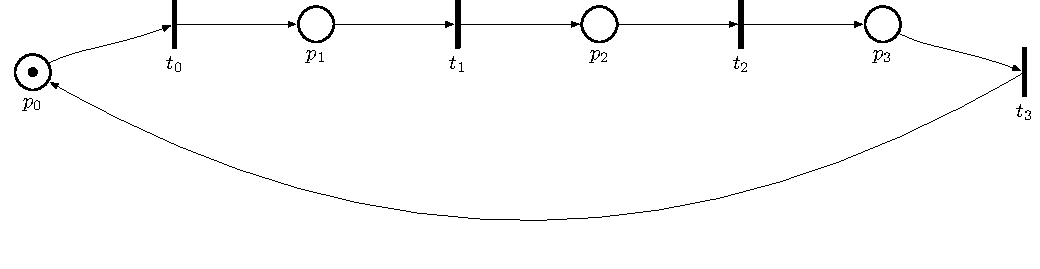
\includegraphics[width=0.8\textwidth]{cipnExample/cipn.tikz}
  \caption[cipnexample]{Example of Control Interpreted Petri Net to control
    system in \autoref{fig:cipnexamplescheme}}
  \label{fig:cipnexample}
\end{figure}

\begin{table}[htbp]
\caption{Control Interpreted Petri Net Example Places.}
\centering
\begin{tabular}{M{5cm}M{10cm}}
Places & Meaning\\
\hline
\hyperlink{cipnExampleNet:p0m1}{\hypertarget{cipnExampleTable:p0m1}{$p_{0}$}} & System Stopped\\
\hyperlink{cipnExampleNet:p1}{\hypertarget{cipnExampleTable:p1}{$p_{1}$}} & R (Car Moving to the Right)\\
\hyperlink{cipnExampleNet:p2}{\hypertarget{cipnExampleTable:p2}{$p_{2}$}} & Open (Container Opened)\\
\hyperlink{cipnExampleNet:p3}{\hypertarget{cipnExampleTable:p3}{$p_{3}$}} & L (Car Moving to the Left)\\
\end{tabular}
\end{table}

\begin{table}[H]
\caption{Control Interpreted Petri Net Example Transitions.}
\centering
\begin{tabular}{M{5cm}M{10cm}}
Transitions & Meaning\\
\hline
\hyperlink{cipnExampleNet:t0}{\hypertarget{cipnExampleTable:t0}{$t_{0}$}} & m (filling request)\\
\hyperlink{cipnExampleNet:t1}{\hypertarget{cipnExampleTable:t1}{$t_{1}$}} & b (Right Limit Switch)\\
\hyperlink{cipnExampleNet:t2}{\hypertarget{cipnExampleTable:t2}{$t_{2}$}} & p (Car is Full)\\
\hyperlink{cipnExampleNet:t3}{\hypertarget{cipnExampleTable:t3}{$t_{3}$}} & a (Left Limit Switch)\\
\end{tabular}
\end{table}

\usetikzlibrary{arrows,shapes,circuits.plc.ladder,external}

\begin{figure}[H]
  \centering
  \includegraphics{cipnExample/cipnLadder.tikz}
  \caption[cipnexample]{Example of Control Interpreted Petri Net converted to Ladder.}
  \label{fig:cipnexampleLadder}
\end{figure}

\begin{figure}[H]
    \centering
    \begin{subfigure}[t]{0.5\textwidth}
      \centering
        \includetikzfigure[width=\textwidth]{communicationPlcPN/communicationPlcPN}
        \caption{Petri Net on PLC 1.}
        \label{fig:communicationPlcPN}
    \end{subfigure}%
    ~ 
    \begin{subfigure}[t]{0.5\textwidth}
        \centering
        \includetikzfigure[width=\textwidth]{communicationPlcPN/communicationPlcPN1}
  \caption{Petri Net on PLC 2.}
  \label{fig:communicationPlcPN1}
    \end{subfigure}
    \caption{Example of Petri Net divided between 2 PLCs.}
\end{figure}


\begin{figure}[H]
    \centering
    \begin{subfigure}[t]{0.45\textwidth}
        \centering
        \includegraphics{communicationPlcPN/communicationPlcPNLadder.tikz}
        \caption{Ladder Logic on PLC 1.}
        \label{fig:communicationPlcPN}
    \end{subfigure}%
\hfill
    \begin{subfigure}[t]{0.45\textwidth}
        \centering
        \includegraphics{communicationPlcPN/communicationPlcPN1Ladder.tikz}
  \caption{Ladder Logic on PLC 2.}
  \label{fig:communicationPlcPN1}
    \end{subfigure}
    \caption{Example of Petri Net divided between 2 PLCs.}
\end{figure}
  

\autoref{fig:communicationPlcPN}

\usetikzlibrary{patterns}
\begin{figure}[H]
  \centering
  \includegraphics[width=0.5\textwidth]{vennDiagramLanguages.tikz}
  \caption{Venn diagram showing relations between $L_{Orig}$, $L_{OrigNI}$,
    $L_{Obs}$, $L_{Exc}$ and $L_{Iden}$}
\end{figure}


%%% Local Variables:
%%% mode: latex
%%% TeX-master: "../monografia.tex"
%%% End: